As it was referred in the \textit{Implementation Plan},  the group committed to implement 4 behaviors for the decoder component. Some of the behaviors were implemented in software, using C++ language, and some implemented adopting some management in hardware, using verilog. The behaviors implemented were:

\begin{itemize}
	\item \textbf{Switch Cases} Decoder (\textit{Sw}).
    \item \textbf{Jump Table} Decoder (\textit{Sw}/\textit{Hw}).
    \item \textbf{Generic} Decoder (\textit{Sw}).
    \item \textbf{Instruction Format} Decoder (\textit{Hw}).
\end{itemize}

In the following sections it will be presented each behavior implemented, along with some relevant code examples and unit tests to prove the proper functioning.


\subsubsubsection{Switch Cases}
The principle of operation is based on \textbf{switch cases}.
The original decoder behavior, present in the reference \textit{DBT}, is also based in switch cases but has always the \textbf{same number of cases per switch case} (listing \ref{lst:old_switchcases}).

\begin{lstlisting} [language=C++, caption=Original Switch Cases Behavior (first switch case)., label=lst:old_switchcases]
void CTranslator8051::decode(uint8_t op){
			uint8_t subOp = op & 0x0F;
			uint8_t regN = op & 0x7;	

			switch(op>>4){
					case 0 :
						fineDecode_0x0(subOp, regN);	break;
					case 1 :
						fineDecode_0x1(subOp, regN);	break; 
     ...   
\end{lstlisting}

For each \texttt{fineDecode\_0x...()} function another switch case is present inside and in each of its cases relies the decoding algorithm for each instruction (listing \ref{lst:old_switchcases2}). Since it is always being used the 4 most significant bits of the opcode for the first switch case and the other 4 bits for the switch cases inside each \texttt{fineDecode\_0x...()} function, the max size of the switchs will be $2^{4}$. So, there are $2^{4}$ \texttt{fineDecode\_0x...()} methods defined.

\begin{lstlisting} [language=C++, caption=Original Switch Cases Behavior (portion of the \texttt{fineDecode\_0x0()} function)., label=lst:old_switchcases2]

void CTranslator8051::fineDecode_0x0(uint8_t subOp, uint8_t Rn)
{
			uint8_t tmp1;
			uint16_t newPC;
		
			switch (subOp) {
					case 0: //NOP
							zprintf("\tNOP\n\n");
	  	break;
					case 1: // AJMP
							tmp1 = FETCH;
							newPC = (env.PC & 0xF800) | 0x0000 | (uint16_t)tmp1; 
	    				gen_writePC(newPC);		
	    				zprintf("\tAJMP 0x%04X\n\n", newPC);
							eoBB = true;		
			break;
		
    ...

\end{lstlisting}

For the new implementation, the idea remains the same, but now it is given the possibility to \textbf{choose the number of bits of the opcode for the evaluation in the switch cases} (point configurable by the user). This way, a more generic approach had to be taken and it will be demonstrated next.

\paragraph{Software Implementation}

\paragraph{}

  In order to ensure a dynamic size for the switch cases what was done was define 256 callback functions ($2^{nBitsOpcode}$, being the nBitsOpcode = 8) to, independently of the user choices, in the end be always called the \texttt{finedecode\_0x...()} function according to the traversal along the switch cases (again, based on the opcode). Listing \ref{lst:new_switchcases} show the current aspect of some \texttt{fineDecode\_0x...()} functions.

\begin{lstlisting} [language=C++, caption=\texttt{fineDecode\_0xe7()} and \texttt{fineDecode\_0xe8()} functions., label=lst:new_switchcases]
void  C8051Arch::fineDecode_0xe7(uint8_t subOp, uint8_t Rn)	// MOV A, @Ri
{   
			target->gen_ld8(tReg2, subOp&0x01 );
  		target->gen_ldi8(tReg1, MEM_BASE, tReg2);
			target->gen_st8(A, tReg1);
			zprintf("\tMOV A, @R%d\n\n", subOp&0x01);  
} 

void  C8051Arch::fineDecode_0xe8(uint8_t subOp, uint8_t Rn)	// MOV A, Rn
{   
			target->gen_ld8(tReg1, Rn); // Load Rn.
			target->gen_st8(A, tReg1);  // Store the value to A.
			zprintf("\tMOV A, R%d\n\n", Rn); 
}
\end{lstlisting}

Now, as it can be seen, the algorithm to decode a specific instruction is inside the respective \texttt{fineDecode\_0x...()} function. So, for example, the instruction whose opcode equals \texttt{0xe8} will "fall" into the \texttt{fineDecode\_0xe8()} callback. Listing \ref{lst:new_switchcases2} shows a portion of the aspect of the switch cases. For the first one is used 7 bits (\texttt{range1}) and for the others 1 bit (\texttt{range2}).

\begin{lstlisting} [language=C++, caption=Portion of the decode function using the Switch Cases behavior., label=lst:new_switchcases2]
void C8051Arch::decode()
{
			uint8_t op = FETCH;
			uint8_t subOp = op & 0x0F;
			uint8_t regN = op & 0x7;
	
			uint8_t range1 = (op >> 1), range2 = (op & 0x1);

			switch  (range1) {
			case 0x0:
	  			switch (range2) {
	  					case 0x0:
	    					fineDecode_0x0(subOp, regN);
	    				break;
	  					case 0x1:
	    					fineDecode_0x1(subOp, regN);
	   					break;
	  			}
			break;
			case 0x1:
	  			switch (range2) {
	  					case 0x0:
	    					fineDecode_0x2(subOp, regN);
	    				break;
	  					case 0x1:
	    					fineDecode_0x3(subOp, regN);
	    				break;
	  			}
			break;
            
	  ...
\end{lstlisting}

Since for the \texttt{range2} is only used the least significant bit of the opcode, the secondary switch cases have only two cases (0 or 1).	 

\paragraph{Unit Tests}

\paragraph{}

In order to test the implemented decoder, a simple test will be presented showing its correct functioning. A basic block was created and stored in memory and the output of the system was logged. This procedure was repeated for several basic block, however, only one example is presented in \ref{fig:teste1_decoder}.   


\begin{figure}[H]
\centerline{
\includegraphics[scale=0.5]{images/teste_decoder1}
}
\caption{Decoder 1 - Unit Test.}
\label{fig:teste1_decoder} 
\end{figure}

As shown, the output was as expected. All instruction that compose the basic block were translated accordingly. The basic block ends in a branch instruction (SJMP).

\subsubsubsection{Jump Table}

Recalling the principle of operation of this type of decoder, it consist in an \textbf{array (table) of pointers to functions} that know how to decode a specific instruction. The opcode serves as index for the table, i.e., if an opcode equals \texttt{0x54}, it will be executed the function whose address is in the position \texttt{0x54} of the table. 


For this decoder behavior, an implementation in \textbf{software}(\textbf{\textit{Sw}}) and one in \textbf{hardware}(\textit{\textbf{Hw}}) was accomplished. Independently of the approach, the \textbf{256 callback functions} ($2^{nBitsOpcode}$, being the nBitsOpcode = 8) were defined. Those callback functions are the same as the ones referred in the Switch Cases decoder, the \texttt{fineDecode\_0x...()} whose job is, once again, take care of a specif instruction. So, the table will contain the addresses of this functions. 

In the hardware approach for this decoder, the behavior its not totally in hardware. The hardware is only a support to theoretically accelerate the process of decode. It will get clear later, in the hardware implementation section.

\paragraph{Software Implementation}

\paragraph{}

Having in mind the idea of the decoder, what was necessary to do first was declare an array (table) of pointers to functions and a typedef as an alias for the pointer. Being \texttt{fineDecode} declared, 256 memory positions of the table were allocated dynamically (listing \ref{lst:jmptable1}). 

\begin{lstlisting} [language=C++, caption= \texttt{JmpTable} declaration, label=lst:jmptable1]
typedef void (C8051Arch::*fineDecode)(uint8_t, uint8_t);
		...
fineDecode *JmpTable;
		...
JmpTable = new fineDecode[NUM_Instructions];
\end{lstlisting}


It was created a new function to initialize the table. So, in the \texttt{initJumpTable()} function, the \texttt{JmpTable} array is filled with the addresses of each \texttt{fineDecode\_0x...()} function. It is possible to visualize a fragment of the function in listing \ref{lst:jmptable2}.   

\begin{lstlisting} [language=C++, caption= \texttt{initJumpTable()} function., label=lst:jmptable2]
void C8051Arch::initJumpTable(){

    JmpTable[0] = &C8051Arch::fineDecode_0x0;
    JmpTable[1] = &C8051Arch::fineDecode_0x1;
    JmpTable[2] = &C8051Arch::fineDecode_0x2;
    JmpTable[3] = &C8051Arch::fineDecode_0x3;
    JmpTable[4] = &C8051Arch::fineDecode_0x4;
    JmpTable[5] = &C8051Arch::fineDecode_0x5;
    JmpTable[6] = &C8051Arch::fineDecode_0x6;
    JmpTable[7] = &C8051Arch::fineDecode_0x7;
    JmpTable[8] = &C8051Arch::fineDecode_0x8;
    JmpTable[9] = &C8051Arch::fineDecode_0x9;
    JmpTable[10] = &C8051Arch::fineDecode_0xa;
    
    ...
\end{lstlisting}

Finally, using the opcode it is possible to access the correct position in the array and execute the respective \texttt{fineDecode\_0x...()} function (listing \ref{lst:jmptable3}).

\begin{lstlisting} [language=C++, caption=Callback function call (\texttt{decode} method)., label=lst:jmptable3]
(this->*(JmpTable[op]))(subOp, regN);
\end{lstlisting}

\paragraph{Software Unit Tests}

\paragraph{}

A unit test was design to validate the jump table implemented in software. It is based in the previous unit test. Figure \ref{fig:teste1_decoder2} shows one basic block being translated.

\begin{figure}[H]
\centerline{
\includegraphics[scale=0.5]{images/teste_decoder2}
}
\caption{Decoder 2 - Unit Test.}
\label{fig:teste1_decoder2} 
\end{figure}

In the example, the basic block ends with a branch instruction (ACALL). In the same way, a set of basic blocks were loaded in memory in order to check if the translation occurs as expected for all cases. 

\paragraph{Hardware Implementation}

\paragraph{}

As mentioned, this hardware implementation serves \textbf{as support} for the software. The only thing that is done in hardware is, after receive the opcode from the software, access to a specific register and \textbf{return} to the software \textbf{the function address to be executed}. This way, it is required to in a first prime, fill an array of registers in the hardware with the \texttt{fineDecode\_0x...()} addresses. The synchronization between the software and the hardware is ensured by means of signals using bits of registers. Also the exchanged data is made through registers. For the \textit{Sw} <-> \textit{Hw} communication, it is used the \textit{AXI} bus.

As it can be seen in listing \ref{lst:hw_jumptable} an \textbf{hardware jump table}, consisting in an array of 256 registers with 32 bits(function address size) each, was created and at every reset event the jump is clean, i.e, filled with zeros (listing \ref{lst:hw_jumptable2}).

\begin{lstlisting} [language=Verilog, caption=Hardware Jump Table., label=lst:hw_jumptable]
reg [`FUNC_SIZE-1 : 0] jmp_table [0 : `TABLE_SIZE-1];
\end{lstlisting}

\begin{lstlisting} [language=Verilog,caption=Jump Table initialization, label=lst:hw_jumptable2]
if(S_AXI_ARESETN == 1'b0)
begin
			for( i = 0 ; i < `TABLE_SIZE ; i = i + 1)
						jmp_table[i] <= 32'h00000000;

			init <= 1'b1;
			index <= 0;         
end
\end{lstlisting}

The software writes the function addresses, one at a time, in a register (\texttt{slv\_reg0}), signals (using the bit 9 of the \texttt{slv\_reg1} in listing \ref{lst:hw_jumptable3}) the hardware and the address stored in the hardware jump table.

\begin{lstlisting} [language=Verilog, caption=Jump Table initialization., label=lst:hw_jumptable3]
if(init == 1'b1 && slv_reg1[9] == 1'b1)
begin
      jmp_table[index] = slv_reg0;
      index = index + 1;
      init <= 1'b0; 
end
\end{lstlisting}

At decode time, the hardware receives the opcode, goes directly to the correct position of the \texttt{jmp\_table} array, writes the address in a register(\texttt{slv\_reg2}) and signals the software to read that register.

\begin{lstlisting} [language=Verilog, caption=Getting the function address., label=lst:hw_jumptable4]
slv_reg2 = jmp_table[slv_reg1[`OPCODE]];

...


if(slv_reg1[8] == 1'b1)
begin           
		slv_reg3 <= 1; 
end
end
\end{lstlisting}

\paragraph{Hardware Unit Tests}

\paragraph{}

To test this hardware implementation, it was used the Vivado environment. So, a testbench was created and it was simulated a request from the software, i.e., simulate a request to obtain a certain function address that is in the hardware register array (table). But first, it was necessary to fill the table and, to make the test easier, the content of each register of the array got the number of the index (simulated function addresses = index of the array).

\begin{figure}[H]
\centerline{
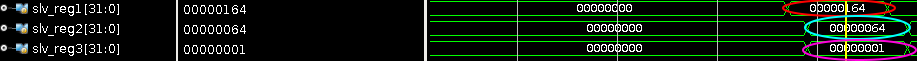
\includegraphics[scale=0.5]{images/test_bench}
}
\caption{Decoder 2 - Hardware Unit Test.}
\label{fig:test_bench} 
\end{figure}

As it can be seen in the figure \ref{fig:test_bench}, that in the red circle there is a simulated opcode (0x64). With that, it can be verified in the blue circle that the simulated function address is 0x64 (equals the index of its position) and the signal to the software (purple circle) is set. 
\subsubsubsection{Generic}

Another behavior proposed in the design phase as a new approach for a decode procedure consists in a generic version of the jump table. However, instead of having a table of callback functions, the table is composed by a structure with information about the steps that must be taken to achieve the target code generations (after decoding the operands).

\paragraph{Software Implementation}

\paragraph{}

The first step in this approach was the definition of the structure. The main idea is to have a \textbf{table} that stores the functions used in the decode process and a \textbf{matrix} that stores references for internal variables used inside those functions. The referred structure is presented in listing \ref{lst:InstructionDecodeSteps}.

\begin{lstlisting} [language=C++, caption= InstructionDecodeSteps structure., label=lst:InstructionDecodeSteps]
typedef void* arg_P;
typedef void (C8051Arch::*method_P)(arg_P*);

struct InstructionDecodeSteps 
{
		method_P* steps;
    arg_P **auxVar;
    int numSteps;
    InstructionDecodeSteps(int numSteps, int numMaxArgs);
};
\end{lstlisting}

As shown, the structure contains a table of type \texttt{method\_P} (\textbf{steps}) and a matrix of type \texttt{arg\_P} (\texttt{auxVar}). The typedef \texttt{method\_P} defines a pointer to a member function of \texttt{C8051Arch} which receives only one argument. This arguments corresponds to a row of the matrix \texttt{auxVar} which contains references to auxiliary variables that shall be used (set/get) inside each method. The table of \texttt{InstructionDecodeSteps} structures with 256 positions were declared as follows:

\begin{lstlisting} [language=C++, caption= InstructionDecodeSteps table declaration., label=lst:generic_jmptable2]
InstructionDecodeSteps** JmpTable;
			...
JmpTable = new InstructionDecodeSteps*[NUM_Instructions];	
\end{lstlisting}

Finally, the table was filled inside the constructor of the class. For that, an exhausting analysis of the decoder code was done. In a generic way, each decode function is composed by a set of generation functions (\texttt{gen\_xx} functions) and auxiliary operations. Since the generation function are already implemented, only new functions were created to implement those operations. Listing \ref{lst:auxMethods} shows the auxiliary methods created.    

\begin{lstlisting} [language=C++, caption= Auxiliary methods, label=lst:auxMethods]
	void fetch(arg_P * ptr);
	void set_eoBB(arg_P * ptr);
	void set_eoExec(arg_P * ptr);
	void AuxFunc_NewPCx(arg_P * ptr);
	void AuxFunc_2bytes(arg_P * ptr);
	void AuxFunc_Ri(arg_P * ptr);
	void AuxFunc_Rn(arg_P * ptr);
	void AuxFunc_ByteAddrAssign(arg_P * ptr);
	void AuxFunc1_0x80(arg_P * ptr);
\end{lstlisting}

As expected, this implementations requires that all steps must have the same signature (one arguement of type \texttt{arg\_P*}). However, the generation functions don not follow this requirement. To overcome this problem, an arrangement was made and wrappers were created around these methods. This approach has a disadvantages since these wrappers increase the overhead. This can be avoided by rewriting every generation function of the target architecture.

\begin{lstlisting} [language=C++, caption = Generation functions., label=lst:gen_generic]
	void gen_movi_wrapper(arg_P * ptr);
	void gen_ld8_wrapper(arg_P * ptr);
	void gen_ldi8_wrapper(arg_P * ptr);
	void gen_st8_wrapper(arg_P * ptr);
	void gen_sti8_wrapper(arg_P * ptr);
  void gen_cje_wrapper(arg_P * ptr);
	void gen_cjne_wrapper(arg_P * ptr);
  
  ...
\end{lstlisting}

Having all methods created, the next step consists in fill all positions of the table. Listing \ref{lst:filltable} illustrates the procedure made for two instruction: \textbf{NOP} and \textbf{AJMP}.

\begin{lstlisting} [language=C++, caption= Initialization of table of structures.
, label=lst:filltable]
	
	// 0x00   NOP
	JmpTable[0x00] = new InstructionDecodeSteps(1, 0);
        JmpTable[0x00]->steps[0] = &C8051Arch::print_NOP;

	//0x01   AJMP
	JmpTable[0x01] = new InstructionDecodeSteps(5, 4);

	JmpTable[0x01]->steps[0] = &C8051Arch::fetch;   //1st step
	JmpTable[0x01]->auxVar[0][0] = &tmp1;           //auxvar1

	JmpTable[0x01]->steps[1] = &C8051Arch::AuxFunc_NewPCx;   //2nd step
	JmpTable[0x01]->auxVar[1][0] = &newPC;                   //auxvar2
	JmpTable[0x01]->auxVar[1][1] = (uint16_t *) &env.PC;     //Src PC
	JmpTable[0x01]->auxVar[1][2] = &v_0x0000;                // 0 
	JmpTable[0x01]->auxVar[1][3] = &tmp1;                    //auxvar1

	JmpTable[0x01]->steps[2] = &C8051Arch::gen_writePC_wrapper;  //3rd step
	JmpTable[0x01]->auxVar[2][0] = &newPC;                    //auxvar2

	JmpTable[0x01]->steps[3] = &C8051Arch::set_eoBB;      //4th step
	JmpTable[0x01]->auxVar[3][0] = (bool *)eoBB;          //eoBB
        
	JmpTable[0x01]->steps[4] = &C8051Arch::print_AJMP;   //5 step
	JmpTable[0x01]->auxVar[4][0] = &newPC;               //debug

	//0x02   LJMP
	
   ...
\end{lstlisting}

Finally, it is presented the decode method for this implementation (listing \ref{lst:decodetable}). Having all steps defined, the method consists in a simple loop through all positions of the step table. 

\begin{lstlisting} [language=C++, caption=Decode method for generic decode behavior.
, label=lst:decodetable]
void C8051Arch::decode()
{
		uint8_t op = FETCH;

    int i, nSteps; v_opcode = op;

    for( i = 0 ; i < JmpTable[op]->numSteps ; i++ )
    {
    	(this->*(JmpTable[op]->steps[i]))(JmpTable[op]->auxVar[i]);
    }      
		return;
}
\end{lstlisting}

\newpage
\paragraph{Unit Tests}

\paragraph{}

The last approach in software was tested in the same way as the others. Another basic block was created and translated for validation purposes. The example is shown in figure \ref{fig:teste1_decoder3}.


\begin{figure}[H]
\centerline{
\includegraphics[scale=0.5]{images/teste_decoder3}
}
\caption{Decoder 3 - Unit Test.}
\label{fig:teste1_decoder3} 
\end{figure}


\subsubsubsection{Instruction Format}

The behavior of this type of decoder is based \textbf{on the format of the instructions}. As known, it was necessary to study the source architecture ISA (8051 ISA) and create groups according to the format. \textbf{Ten groups were created}. This way, when the opcode is acquired, and accordingly to its group, the \textbf{operands are obtained}. 

\paragraph{Hardware Implementation}

\paragraph{}

Like the hardware implementation of the Jump Table decoder, this current hardware implementation also serves \textbf{as support for the software}. Basically, the complete instruction is received from the software, the opcode is analyzed and according to the group, the operands are obtained and stored in a register for the software.

Since the existence of ten groups, \textbf{it was created ten tasks} in which each one is prepared to deal with a specific instruction format. Listing \ref{lst:decode_format} shows some of that tasks.

\begin{lstlisting} [language=Verilog, caption=Group 5 and 6 tasks, label=lst:decode_format]
task TGroup5;
begin
    slv_reg1[`OPERATION] = slv_reg0[`OPERATION_TYPE4];
    slv_reg1[`OP1] = slv_reg0[`BYTE2];
    slv_reg1[`OP2] = slv_reg0[`ADDR11_3BITS];
    slv_reg2 = {1'b1, `GROUP5};
end
endtask
    
task TGroup6;
begin
    slv_reg1[`OPERATION] = slv_reg0[`OPERATION_TYPE2];
    slv_reg1[`OP1] = slv_reg0[`Rn];
    slv_reg1[`OP2] = slv_reg0[`BYTE2];
    slv_reg2 = {1'b1, `GROUP6};
end
endtask
\end{lstlisting}

When the software fetches all the instruction, it \textbf{signals} the hardware and \textbf{sends it the instruction}. Then, what the hardware needs to do is to discover to which group belongs that opcode and call the respective task (listing \ref{lst:decode_format3}). 

\begin{lstlisting} [language=Verilog, caption=Fragment of the \texttt{FGroup\_Selection()} task.
, label=lst:decode_format2]
task FGroup_Selection;
input [7:0] opcode;
output [3:0] group;
  
begin
		case (opcode)
      `NOP,`RR,`INC_A,`RRC,`DEC_A,`RL,`RLC,`RET,`RETI,`JMP, 
      `MOVC_A_PC,`DIV, `MOVC_A_DPTR, `INC_DPTR,`MUL, `CPL_C,
      `CLR_C,`SWAP,`SETB_C, `DA, `MOVX_A_DPTR, `CLR_A, `MOVX_DPTR_A,
      `CPL_A  : group = `GROUP1;
      
	...
\end{lstlisting}

To discover to which group belongs the opcode, it was created a task, \texttt{FGroup\_Selection()} that contains a big switch case involving all the opcodes organized by group (listing \ref{lst:decode_format2}). Depending on the group, the variable \texttt{group\_select} gets the value corresponding to the number of the group. From here it is \textbf{called the respective group} task which splits the instructions and stores the fields in the \texttt{slv\_reg1} register (listing \ref{lst:decode_format}). Also the number of the group is sent to the software in order to be recognized the group of the instruction and be called a specific function.



\begin{lstlisting} [language=Verilog, caption=Selection of the group task.
, label=lst:decode_format3]
FGroup_Selection(slv_reg0[`OPCODE], group_select);        
           
case (group_select)
      `GROUP1:  TGroup1;
      `GROUP2:  TGroup2;
      `GROUP3:  TGroup3;
      `GROUP4:  TGroup4;
      `GROUP5:  TGroup5;
      `GROUP6:  TGroup6;
      `GROUP7:  TGroup7;
      `GROUP8:  TGroup8;
      `GROUP9:  TGroup9;
      `GROUP10: TGroup10;          
endcase
\end{lstlisting}



